\chapter{Návrh programu}

\label{kap:design} % id kapitoly pre prikaz ref

V návrhu bakalárskej práce vystupujú rôzne entity medzi ktorými sú rôzne vzťahy. 
\begin{figure}[H]
\centerline{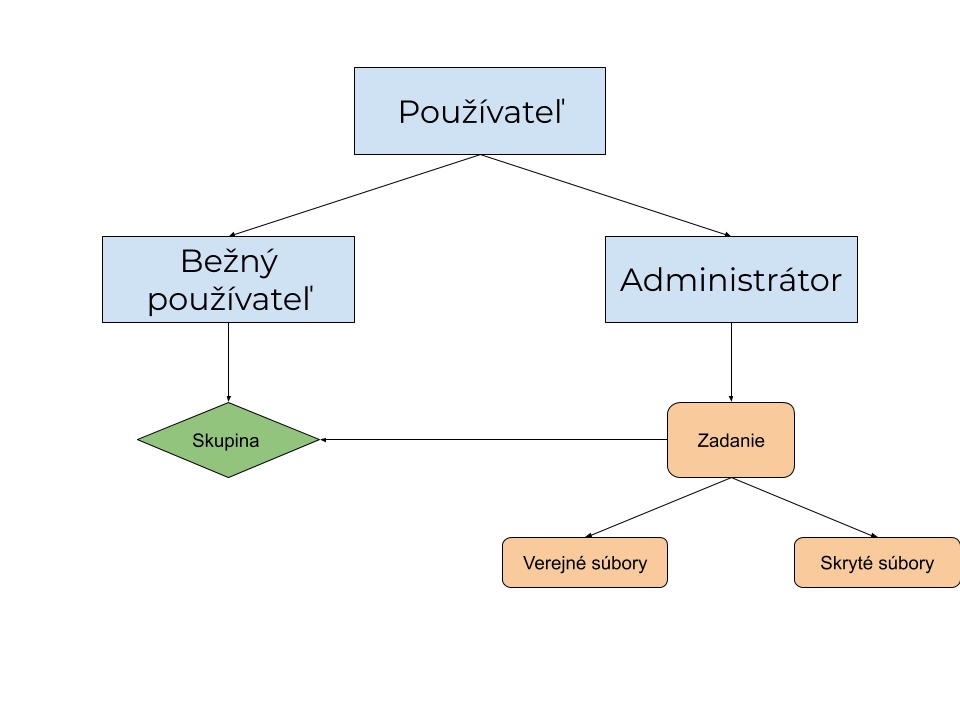
\includegraphics[width=1\textwidth]{images/entity}}
\caption[Entity v návrhu]{Entity v návrhu}
\label{obr:entity}
\end{figure}

\begin{description}
\item [Používateľ] - Entita, pomenúvajúca používateľa aplikácie. Používateľov rozdeľujeme na 
bežných používateľov a administrátorov.
\item [Bežný používateľ] - Bežní používatelia predstavujú zovšeobecnený pojem pre študentov. Každý
bežný používateľ patrí do niekoľkých skupín, v ktorých má prístup iba k úlohám prístupným pre danú
skupinu.
\item [Administrátor] - Administrátor má plný prístup ku všetkým informáciám na serveri. Okrem
toho pridáva bežných používateľov do skupín, pridáva zadania, vidí odovzdané zadania bežných
používateľov...
\item [Skupina] - Skupina je enita, ktorá sa skladá bežných používateľov. Každé zadanie musí
patriť do práve jednej skupiny. Toto zadanie je prístupné iba pre používateľov, ktorý patria do
danej skupiny. 
\item [Zadanie] - Administrátor vie vytvoriť zadanie pre nejakú skupinu, ktoré môžu bežní
používatelia riešiť. Zadanie obsahuje verejné a skryté súbory.
\item [Verejné súbory] - Verejné súbory, sú súbory zadania, ktoré sú prístupné pre klienta.
\item [Skryté súbory] - Skryté súbory by nikdy nemali byť posielané na klienta, a slúžia na 
vytvorenie skrytých vstupov a správnych riešení, prípadne iných súborov, ku ktorým by klient
nemal mať prístup.
\end{description}

Program sa skladá z viacerých častí, ktorých návrhy popíšeme v tejto kapitole.
Návrh je založený na klient-server architektúre. Program sa preto dá rozdeliť na 
podkapitoly \textit{klient} a \textit{server}.

\section{Klient}
Klient je v bakalárskej práci webová aplikácia cez ktorú používateľ komunikuje so serverom. V návrhu
klienta sa snažíme hlavne vytvoriť jednoduché používateľské prostredie, ktoré je intuitívne na
použitie. Kedže aplikácia má byť používaná ako editor, je nutné aby sa jednotlivé časti pohodlne
čítali a písmo bolo dostatočne veľké. Naopak, nepredpokladáme použitie editora na mobilných
zariadeniach. Preto je dizajn klienta tvorený pre použitie na počítačoch a na veľkých obrazovkách.
Klientská aplikácia obsahuje:
\begin{itemize}
\item rozhranie pre prihlasovanie a registráciu
\item administrátorské rozhranie
\item rozhranie pre bežného používateľa
\end{itemize}

\subsection{Prihlasovanie a registrácia}
Prihlasovanie slúži na jednoduché kategorizovanie používateľa a na prístup k editoru. Každý
používateľ má svoje prihlasovacie meno a heslo, pod ktorým sa zaregistroval. Prihlasovanie a
registrácia sú pre oba typy používateľov rovnaké.

Registrácia umožňuje vytvoriť nového používateľa. Zaujímavá otázka je, či umožniť vytváranie
administrátorov priamo pri regsitrácii, alebo nejakým iným spôsobom. Rozhodli sme sa, že je lepšie
ak používateľ nemusí pri registrácii riešiť koncept administrátorov, a teda umožniť iba vytváranie
bežných používateľov. 

\subsection{Administrátorské rozhranie}
Po prihlásení sa administrátorovi automaticky zobrazí administrátorské rozhranie, ktoré je rozdielne
od rozhrania pre bežného používateľa. Adminstrátorské rozhranie umožňuje:
\begin{itemize}
\item zobraziť, upraviť a odstrániť používateľa
\item zobraziť všetky uložené zadania
\item zobraziť všetky odovzdané zadania
\item vytvoriť, upraviť a odstrániť zadanie
\item pridať, upraviť a odstrániť skupiny
\end{itemize}

\subsection{Rozhranie pre bežného používateľa}
Rozhranie pre bežného používateľa slúži iba nato aby si používateľ mohol vybrať skupinu a zadanie,
na ktorom chce pracovať. Po zvolení zadania sa zobrazí editor, v ktorom môže používateľ zadanie
riešiť. Editor sa automaticky synchronizuje na vzdialených počítačoch, prípadne nových kartách 
vo webovom prehliadači. Synchronozácia je granulovaná pre používateľa. To znamená, že ak sa dva
počítače navzájom synchronizujú, sú práve prihlásené pod tým istým používateľom.

% https://tex.stackexchange.com/questions/5035/paragraph-style-how-to-force-line-break-paragraph-make-paragraph-a-he
\paragraph{Panel so súbormi}\leavevmode\\
Úlohy sa môžu skladať z viacerých súborov. Napríklad môže existovať súbor, ktorý
obsahuje zadanie a súbor (prípadne viac súborov) na zdrojový kód. Panel so súbormi dovoľuje
používateľovi pohodlne preklikávať a zvoliť aktívny súbor, ktorý sa zobrazuje v editore.

% https://tex.stackexchange.com/questions/5035/paragraph-style-how-to-force-line-break-paragraph-make-paragraph-a-he
\paragraph{Zdieľateľný editor}\leavevmode\\
Najzaujímavejšou častou práce je kolaboratívny editor umožnujúci bežným používateľom naraz
upravovať kód. V editore musí byť jasné, ktorý súbor sa práve upravuje a bolo by
tiež dobré vedieť nejaké informácie o vzdialených používaťeloch ako napríklad prihlasovacie meno, 
pozícia kurzora...

% https://tex.stackexchange.com/questions/5035/paragraph-style-how-to-force-line-break-paragraph-make-paragraph-a-he
\paragraph{Ovládací panel}\leavevmode\\
Samotná úprava kódu je dôležitá, ale okrem toho je potrebné verzionovanie
súborov, teda nejaké ukladanie a načítavanie. Okrem toho by používateľ mal mať možnost práve
upravovaný kód spúštať na vlastnom vstupe alebo na skrytých vstupoch danej úlohy.


\section{Server}
Server slúži na komunikáciu s klientom a obsahuje všetky potrebné informácie o používateľoch,
administrátoroch, skupinách a vytvorených zadaniach.

Server má viacero funkcií:
\begin{itemize}
\item synchronizácia replík klientov
\item uchovávať informácie o používateľoch a zadaniach
\item poskytovať API pre klienta
\item zbiehanie kódu, poskytovanie odpovede klientom
\end{itemize}

\subsection{Synchronozácia replík klientov}
Najdôležitejšou funckiou servera je synchronizácia replík klientov ak nastane nejaká zmena
dokumentu. Server na toto nepotrebuje veľkú logiku, ale potrebuje korektne preposielať informácie
medzi klientami a reagovať na prípadné komunikačné chyby (odoslať správu znovu).

\subsection{Uchovávať informácie o používateľoch a zadaniach}
Po registrácii sa musia na serveri uložiť informácie o používateľovi, aby sa následne mohol opätovne
prihlasovať. Okrem toho klient môže ukladať a načítavať zadania, ktoré tiež musia byť nejakým
spôsobom na serveri uložené.

\subsection{Poskytovať API pre klienta}
Hlavnou funckiou servera je poskytovať API rozhranie, ktoré môže klient zavolať a vykonať nejakú
akciu na serveri. Časť rozhrania služi na získanie informácií zo servera a čast vytvára
na serveri nové položky (používatelia, zadania).

\subsection{Zbiehanie kódu, poskytovanie odpovede klientom}
Kód, ktorý sa napíše na klientoch sa má dať spustiť v izolovanom prostredí servera. Aplikácia by
mala poskytnúť dve možnosti ako testovať klientský kód:
\begin{itemize}
\item na vlastnom vstupe
\item na skrytých vstupoch
\end{itemize}

Pri testovaní na vlastnom vstupe by používateľ na klientovi mal mať možnosť zadať vstup a potom
odoslať požiadavku na testovanie serveru. Po otestovaní by sa mal klientovi zobraziť výsledok
testovania. Testovanie na vlastných vstupoch nemusí byť ukladané na serveri, stačí ak server na
požiadavku odpovie. Ak by výsledok testovania skončil chybou pri kompilácii, prípadne chybou počas
behu programu, daná chybová hláška sa má zobraziť ako výstup programu.

Okrem testovania na vlastných vstupoch si vie používateľ otestovať kód aj na skrytých vstupoch a
výstupoch zadania. Takéto skryté vstupy vie pridať iba administrátor a nikdy by nemali byť zobrazené
bežnému používateľovi. Každé testovanie na skrytých vstupoch musí byť uložené na serveri, aby si ho
administrátor vedel pozrieť keď bude ohodnocovať dané zadanie bežného používateľa. Po odoslaní
požiadavky serveru na otestovanie na skrytých vstupoch by sa mali zobraziť výsledky testovania.
Skrytých vstupov môže byť viac, ale testuje sa na vstupoch zaradom a keď sa nájde vstup, na ktorom
program dáva nesprávny výstup, tak sa v testovaní ďalej nepokračuje.
Výsledok testovania jedného vstupu môže byť:
\begin{itemize}
\item OK - Kompilácia a aj beh programu prebehli v poriadku a výsledok programu na danom vstupe
je totožný so správnym výstupom
\item WA - Kompilácia prebehla v poriadku a program úspešne skončil, ale výstup sa nezhoduje so
správnym výstupom
\item TLE - Kompilácia prebehla v poriadku, ale program prekročil časový limit, ktorý je dostupný 
pre dané zadanie.
\item RTE - Kompilácia prebehla v poriadku, ale program počas behu programu spadol.
\item CE - Kompilácia programu sa nepodarila.
\end{itemize}
\textit{(V prípade, že jazyk, v ktorom je kód napísaný je interpretovaný, sa kompilácia preskakuje.
Stále však môžu nastať všetky výsledky testovania s výnimkou CE)}
